% We import package amsmath before the documentclass to avoid the warning.
% Command '\usepackage{amsmath}' results in the following warning:
% Package amsmath Warning: Unable to redefine math accent \vec.
\RequirePackage{amsmath} % for environments such as align

\def\mode{1} % 0: Graduation thesis, 1: ICPR paper

\ifnum\mode=0
  \documentclass[11pt]{article}
  \usepackage{luatexja}
  \usepackage{style/prmlthesis}
  \usepackage[a4paper]{geometry}
\else
  \documentclass[runningheads]{llncs}
\fi

% If possible, figure files should be included in EPS format.

% If you use the hyperref package, please uncomment the following two lines
% to display URLs in blue roman font according to Springer's eBook style:
%\usepackage{color}
%\renewcommand\UrlFont{\color{blue}\rmfamily}

% The following code is used to remove the warning with subcaption package:
% ------------------------------
% Package caption Warning: Unknown document class (or package),
% standard defaults will be used.
% ------------------------------
% cf. https://teratail.com/questions/q2vuwf6skm5hph
\makeatletter
\def\caption@documentclass{elsarticle}
\makeatother

\usepackage{algorithm}
\usepackage{algpseudocode}
\usepackage{amssymb} % for \mathbb
\usepackage{array} % for m column type
\usepackage{bbm} % for \mathbbm
\usepackage{booktabs} % for \toprule, \midrule, \bottomrule
\usepackage{cleveref} % for \cref
\usepackage{csvsimple} % for \csvreader
\usepackage[T1]{fontenc} % for T1 font encoding
\usepackage{graphicx} % for \includegraphics
\usepackage{pgffor} % for \foreach
\usepackage[labelformat=simple]{subcaption} % for subfigure environment
\usepackage{tikz}
\usetikzlibrary{positioning}

% The following code is used to remove the warning with bibliography:
% ------------------------------
% Underfull \hbox (badness 2653) in paragraph at lines 28--34
% ------------------------------
% cf. https://tex.stackexchange.com/questions/10924/underfull-hbox-in-bibliography
\apptocmd{\sloppy}{\hbadness 10000\relax}{}{}

% set the path for figures
\graphicspath{{./src/}{../python/data/}{../experiments/}}

% set the label format for subcaption
\renewcommand\thesubfigure{(\alph{subfigure})}

% settings for cleveref
\crefname{table}{Table}{Tables}
\crefname{algorithm}{Algorithm}{Algorithms}
\ifnum\mode=0
  \crefname{figure}{Figure}{Figures}
\else
  \crefname{figure}{Fig.}{Figs.}
\fi

% import the TeX file containing macro definitions
\newcommand{\ispace}{\mathbb{D}^{m}}
\newcommand{\Prec}{\operatorname{acc}}
\newcommand{\Cov}{\operatorname{cov}}
\newcommand{\cands}{\bar{\mathcal{A}}}
\algnewcommand{\IIf}[1]{\State\algorithmicif\ #1\ \algorithmicthen\ }
\renewcommand{\algorithmicrequire}{\textbf{Input:}}
\renewcommand{\algorithmicensure}{\textbf{Output:}}


\begin{document}

\ifnum\mode=0
  \title{%
    R-LIME: LIME法における矩形制約と最適化
  }
  \etitle{%
    R-LIME: Rectangular Constraints and Optimization for Local Interpretable
    Model-agnostic Explanation Methods
  }
  \author{大原 玄嗣 (Genji Ohara)}
  \institute{%
    北海道大学 工学部 \\
    情報エレクトロニクス学科 \\
    情報理工学コース \\
    情報認識学研究室
  }
  \date{2024年3月}
  % \institute{%
  %   Laboratory for Pattern Recognition and Machine Learning,\\
  %   Division of Computer Science and Information Technology,\\
  %   Department of Electronics and Information Engineering,\\
  %   School of Engineering, Hokkaido University
  % }
\else
  % The title of the paper
  \title{%
    R-LIME: Rectangular Constraints and Optimization for Local Interpretable
    Model-agnostic Explanation Methods
  }

  % Abbreviated title for the running head
  \titlerunning{%
    R-LIME: Rectangular Constraints and Optimization for LIME Methods
  }

  % Author names and ORCID IDs
  \author{Genji Ohara\orcidID{0009-0000-5854-2820} \and
    Keigo Kimura\orcidID{0000-0002-3614-6568} \and
    Mineichi Kudo\orcidID{0000-0003-1013-3870}
  }

  % Abbreviated author list for the running head (First names are abbreviated)
  % If there are more than two authors, 'et al.' is used.
  \authorrunning{G. Ohara et al.}

  % The authors' affiliations
  \institute{Division of Computer Science and Information Technology\\
    Graduate School of Information Sci.\ and Tech.,
    Hokkaido University\\
    Sapporo 060-0814, JAPAN,\\
    \email{\{genji-ohara, kimura5, mine\}@ist.hokudai.ac.jp}}
\fi

% typeset the header of the contribution
\maketitle              %

\ifnum\mode=0
  \pagestyle{plain}
  \pagenumbering{roman}
  \tableofcontents
  \newpage
  \listoffigures\listoftables\clearpage
  \AddToHook{cmd/section/before}{\clearpage}
  \pagestyle{plain}
  \pagenumbering{arabic}
\else
  % The abstract should briefly summarize the contents of the paper in
  % 150--250 words.
  \begin{abstract}
    In recent years,
    complex machine learning models have been introduced
    in various industrial fields due to their high accuracy.
    However,
    their complexity has been a major obstacle to implementation
    in sensitive decision-making situations.
    In order to address this problem,
    various post-hoc explanation methods have been proposed,
    but they have not been able to achieve interpretability of
    both the explanation and its scope.
    We propose a new method, R-LIME,
    which interprets complex classifiers in an interpretable scope.
    R-LIME locally approximates a decision boundary of a black-box classifier
    in a rectangular region
    and maximizes the region as long as the accuracy of the linear
    classifier is higher than a given threshold.
    The resulting rectangular region is interpretable for users because it is
    expressed as a conjunction of feature predicates.
    Comparing R-LIME with the existing method,
    we demonstrate the effectiveness of the proposed method through qualitative
    and quantitative experiments using a real-world dataset.
    % 150 words
    \keywords{Interpretable machine learning \and Local surrogate model}
  \end{abstract}
\fi

\section{Introduction}
Machine learning models, such as deep learning and random forests,
have been widely employed in various industrial applications
due to their significant improvement in accuracy in recent years.
However,
the increasing complexity and black-box nature of these models pose challenges,
particularly in critical decision-making scenarios like healthcare and finance,
where the opacity of decision process becomes a major obstacle to
implementation.
Consequently,
there has been extensive research in the field of post-hoc explanations
for machine learning models~\cite{%
  guidotti2018local,radulovic2023bella,ribeiro2016why,ribeiro2018anchors}.
Existing post-hoc explanation methods are categorized
into \emph{model-dependent} and \emph{model-agnostic} methods
based on their dependence on the model's structure.
Furthermore, model-agnostic methods are classified into
\emph{global} and \emph{local} methods based on their locality in input space.
\begin{figure}[tbp]
  \def\scale{0.38}
  \centering
  \begin{subfigure}[t]{0.55\textwidth}
    \centering
    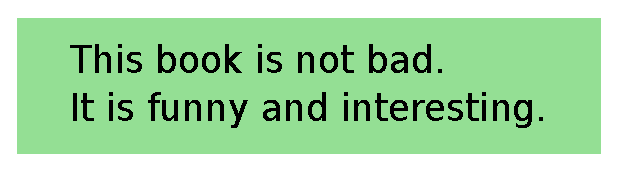
\includegraphics[scale=\scale]{example-instance}
    \caption{Focal point.}\label{fig:example-instance}
    \vspace{0.5cm}
  \end{subfigure}
  \begin{subfigure}[t]{0.45\textwidth}
    \begin{subfigure}[t]{\textwidth}
      \centering
      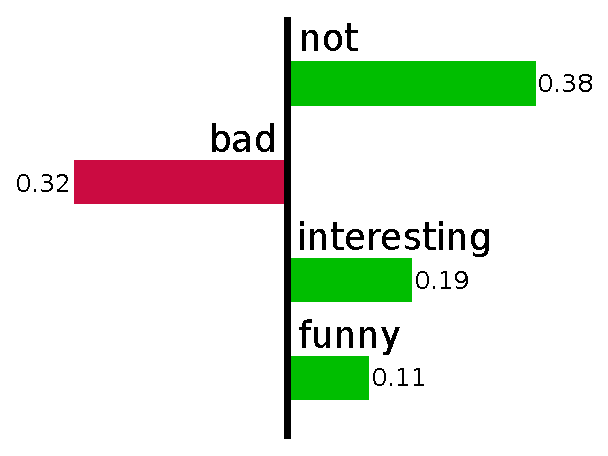
\includegraphics[scale=\scale]{example-lime}
      \caption{%
        Explanation by LIME\@.
        It provides contributions of each feature to the output,
        but does not explicitly indicate its scope.
      }\label{fig:example-lime}
      \vspace{0.4cm}
    \end{subfigure}
    \begin{subfigure}[t]{\textwidth}
      \centering
      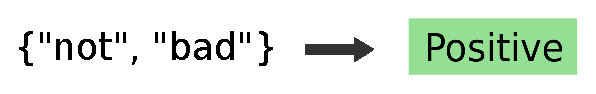
\includegraphics[scale=\scale]{example-anchor}
      \caption{%
        Explanation by Anchor.
        It provides the effective scope of the explanation,
        but does not show the influence of each feature.
      }\label{fig:example-anchor}
    \end{subfigure}
  \end{subfigure}
  \hspace{0.3cm}
  \begin{subfigure}[t]{0.45\textwidth}
    \centering
    \ifnum\mode=0
      \vspace{-1.79cm}
    \else
      \vspace{-2.24cm}
    \fi
    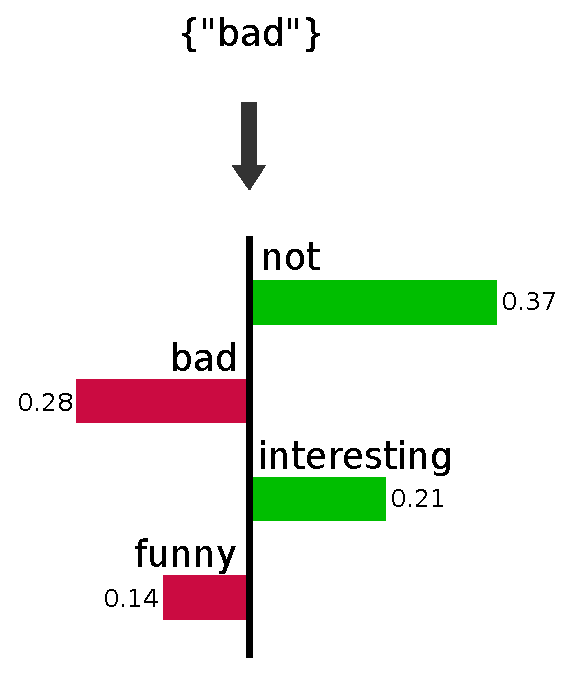
\includegraphics[scale=\scale]{example-rlime}
    \caption{%
      Explanation by R-LIME\@.
      It provides both contributions of each feature and
      its effective scope.
    }\label{fig:example-rlime}
  \end{subfigure}
  \caption[Example of explanations by LIME, Anchor and R-LIME]{%
    Example of explanations by LIME~\cite{ribeiro2016why},
    Anchor~\cite{ribeiro2018anchors} and R-LIME (our proposed method).
    for a sentiment prediction model.
  }\label{fig:example}
\end{figure}

In this paper,
we focus on local model-agnostic methods.
An example of explanations by LIME~\cite{ribeiro2016why} and
Anchor~\cite{ribeiro2018anchors}
for a sentiment prediction model is illustrated in \cref{fig:example}.
LIME approximates the complex decision boundary
linearly around the given focal point,
then provides the weights of the linear model as the contribution of each feature
to the output.
The explanation by LIME (\cref{fig:example-lime}) provides suggests that
the word ``not'' mainly contributes to the positive prediction,
but does not explicitly indicate the effective scope.
Without the scope,
users might mistakenly apply the knowledge derived from the explanation
to other instances far from the focal point,
potentially leading to misunderstanding of the black-box model's behavior
\cite{ribeiro2018anchors}.
For this example,
user may apply the derived insights
to the sentence ``This book is not good.''
and mistakenly conclude that the word ``not''
mainly contributes to the positive prediction for this sentence as well,
which is obviously incorrect.
Anchor represents a rectangular region
containing the focal point,
that maximizes the probability of the black-box classifier outputting
the same label as the focal point.
While Anchor provides an effective scope of the explanation,
the information it includes is less than LIME,
limiting its utility~\cite{ribeiro2018anchors}.
The explanation by Anchor (\cref{fig:example-anchor})
suggests that changing words other than ``not'' and ``bad''
has little impact on the classifier's output.
While it clearly cannot be applied to the sentence ``This book is not good''
because of not including the word ``bad'',
the explanation does not provide details about the influence of each word,
resulting in less user insight into the model's behavior compared to LIME.

To address this limitation of LIME,
we propose a new method called R-LIME (Ruled LIME),
which interprets complex classifiers in an interpretable region.
R-LIME locally approximates a complex decision boundary linearly
in a rectangular region and maximizes the region
as long as the accuracy of the linear classifier is
higher than a given threshold.
The rectangular region is interpretable for users because it is
expressed as a conjunction of feature predicates (\cref{fig:example-rlime}).
An example of the explanation by R-LIME for a sentiment prediction model
is illustrated in \cref{fig:example-rlime}.
It is clear that users can apply the insights derived from the explanation
only to the sentences containing the word ``not''.

\section{Related Work}
\begin{figure}[tbp]
  \centering
  \def\w{2.5}
  \def\ww{5.0}
  \def\h{0.7}
  \def\hh{1.4}
  \def\hhh{2.1}
  \def\hhhh{2.8}
  \begin{tikzpicture}[scale=0.9,nodestyle/.style={rectangle,auto}]
    \node[nodestyle] (post-hoc) at (0,0){post-hoc};
    \node[nodestyle] (dependent) at (-\w,-\hh){%
      \begin{tabular}{c}
        model-dependent \\
        (DTD~\cite{montavon2017explaining}, LRP~\cite{bach2015pixel})
      \end{tabular}
    };
    \node[nodestyle] (agnostic) at (\w,-\hh){\textbf{model-agnostic}};
    \node[nodestyle] (global) at (0,-\hhhh){%
      \begin{tabular}{c}
        global \\
        (PDP~\cite{friedman2001greedy}, ALE~\cite{apley2020visualizing})
      \end{tabular}
    };
    \node[nodestyle] (local) at (\ww,-\hhhh){%
      \begin{tabular}{c}
        \textbf{local} \\
        (LIME~\cite{ribeiro2016why}, Anchor~\cite{ribeiro2018anchors}, \underline{R-LIME})
      \end{tabular}
    };
    \draw(post-hoc) -- (0,-\h);
    \draw(dependent) -- (-\w,-\h) -- (\w,-\h) -- (agnostic);
    \draw(agnostic) -- (\w,-\hhh);
    \draw(global) -- (0,-\hhh)  -- (\ww,-\hhh) -- (local);
  \end{tikzpicture}
  \caption{%
    Categorization of post-hoc explanation methods.
    We focus on \emph{model-agnostic} and \emph{local} methods,
    which explain model's local behavior using only its output.
  }\label{fig:post-hoc}
\end{figure}
In this section,
we overview existing research on post-hoc explanation methods,
which explain the behavior of black-box models already trained.
As shown in \cref{fig:post-hoc},
post-hoc methods are classified into several categories.

They are broadly divided into
\emph{model-dependent} and \emph{model-agnostic} methods
based on their dependence on the model's structure.
Model-dependent methods,
such as Deep Taylor Decomposition (DTD)~\cite{montavon2017explaining}
and Layer-wise Relevance Propagation (LRP)~\cite{bach2015pixel},
most of which focus on neural networks and
explain the model's behavior using its parameters~\cite{samek2021explaining}.
While these methods provide detailed explanations
(e.g., layer-wise explanations for neural networks),
it is often challenging
to apply the same method to models with different structures.
On the other hand,
model-agnostic methods use only the output of the model.
Although they are applicable to any model,
they cannot explain the reasoning process inside the model.

Furthermore, model-agnostic methods are categorized into
\emph{global} and \emph{local} methods based on their locality in input space.
Global methods,
such as Partial Dependence Plots (PDP)~\cite{friedman2001greedy}
and Accumulated Local Effects (ALE)~\cite{apley2020visualizing},
aim to explain the model's behavior across the entire input space.
% seeking explanations valid for any input.
However, providing global explanations becomes challenging
as the model's complexity increases.
In contrast, local methods,
such as Local Interpretable Model-agnostic Explanations (LIME)
\cite{ribeiro2016why}
and Anchor~\cite{ribeiro2018anchors},
% SHAP~\cite{lundberg2017unified},
% EXPLAN~\cite{rasouli2020explan},
% LORE (Local Rule-based Explanations)~\cite{guidotti2018local}
% and BELLA (Black box model Explanations by Local Linear Approximations)
% \cite{radulovic2023bella},
explain model's behavior in the vicinity of a specific input.
While local methods offer explanations more simple and accurate
than global methods,
the scope of the explanation is limited locally.

\section{Proposed Method}
\begin{figure}[tbp]
  \centering
  \begin{subfigure}[t]{0.3\textwidth}
    \centering
    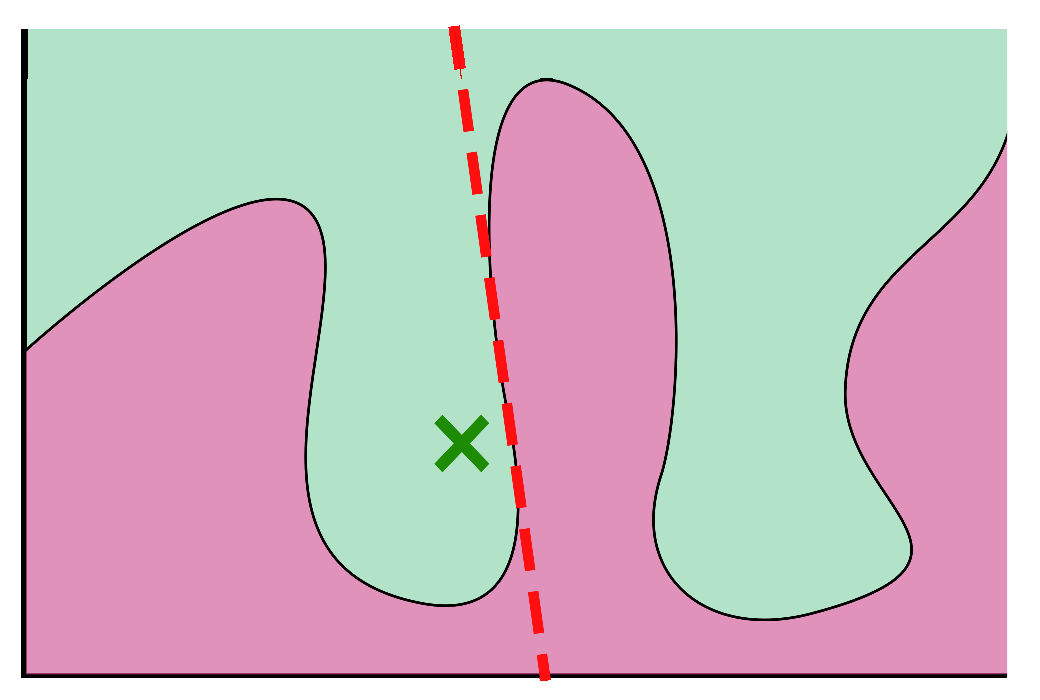
\includegraphics[width=\textwidth]{visual-lime}
    \caption{%
      LIME: Locally approximates the decision boundary around the focal point.
    }\label{fig:lime}
  \end{subfigure}%
  \hspace{0.03\textwidth}
  \begin{subfigure}[t]{0.3\textwidth}
    \centering
    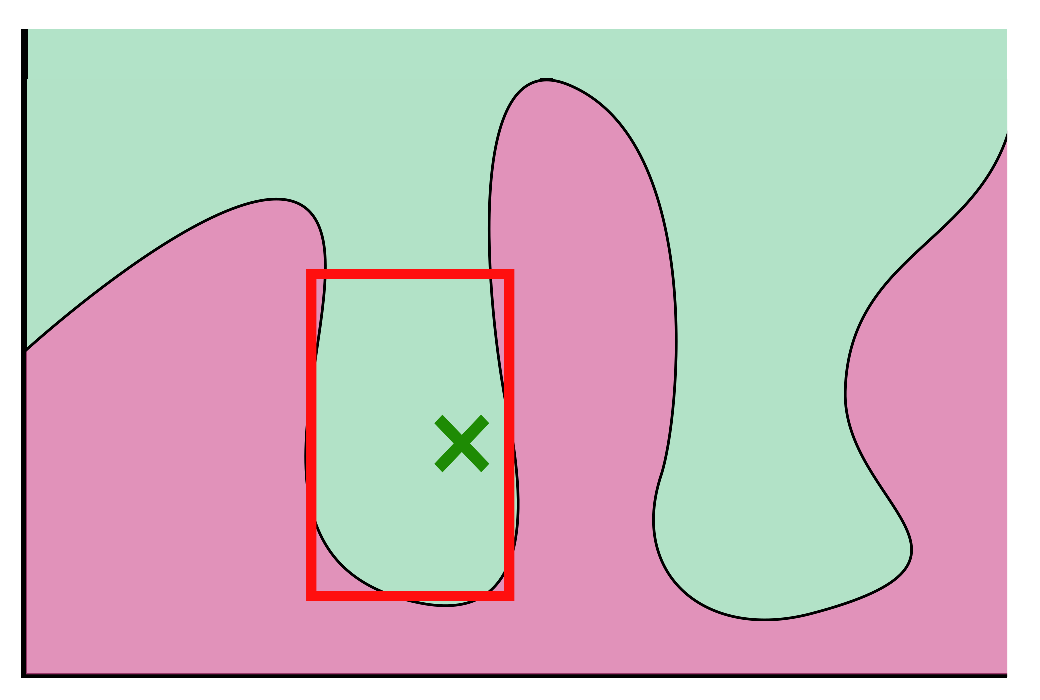
\includegraphics[width=\textwidth]{visual-anchor}
    \caption{%
      Anchor: Maximizes coverage of a rectangular region
      containing the focal point under accuracy constraints.
    }\label{fig:anchor}
  \end{subfigure}
  \hspace{0.03\textwidth}
  \begin{subfigure}[t]{0.3\textwidth}
    \centering
    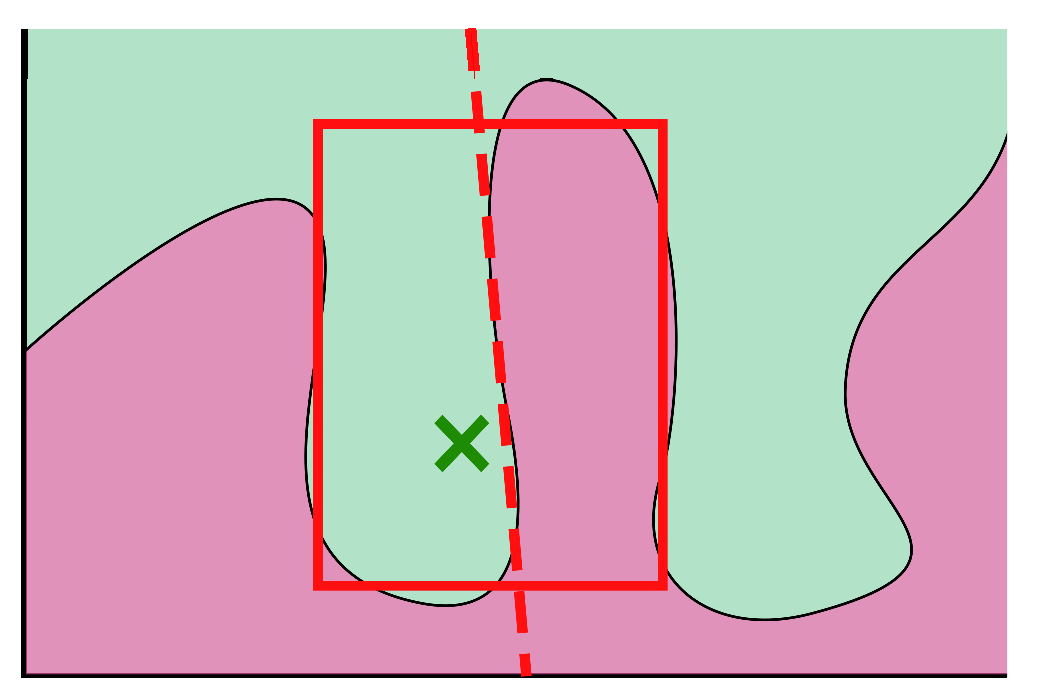
\includegraphics[width=\textwidth]{visual-rlime3}
    \caption{%
      R-LIME:
      Maximizes coverage of a rectangular region
      under lower constraints on the accuracy of the linear classifier.
    }\label{fig:rlime}
  \end{subfigure}
  \caption[Visual comparison of LIME, Anchor and R-LIME]{%
    Visual comparison of LIME, Anchor and R-LIME (our proposed method).
    The solid line represents the rectangular region containing the focal
    point, and the dashed line represents the learned approximation model.
  }
\end{figure}

\subsection{Previous Work}
We specifically focus on \emph{local} and \emph{model-agnostic} methods.
In this section,
we briefly review existing research on local model-agnostic explanations,
particularly focusing on studies closely related to our proposed method.

\subsubsection[LIME]{%
  LIME (Local Interpretable Model-agnostic Explanations)
  \cite{ribeiro2016why}
}
LIME locally
approximates a black-box classifier $f: \mathbb{R}^m \to \{0,1\}$
around a focal point $x \in \mathbb{R}^m$
by a linear classifier $g: \mathbb{R}^m \to \{0,1\}$
(\cref{fig:lime}).
The approximation is performed by the following two steps:
\begin{enumerate}
  \item Generating a set of perturbed samples $\mathcal{Z}_p$ around $x$
        and the set of pseudo-labels $f(\mathcal{Z}_p) = \{f(z) \mid z \in \mathcal{Z}_p\}$.
        (i) $x$ is converted into a binary vector
        $x'\in\{0,1\}^{m'}$,
        (ii) perturbed samples are generated by drawing non-zero elements
        from $x'$ uniformly at random,
        and (iii) the perturbed samples are converted back to the original space.
  \item Learning a linear classifier $g$
        using $\mathcal{Z}_p$ and $f(\mathcal{Z}_p)$
        by minimizing the following loss function:
        \begin{equation}
          \label{eq:lime_loss}
          \mathcal{L}(f,g,\pi_x)=\sum_{z\in\mathcal{Z}_p}
          \pi_x(z){\left(f(z)-g(z)\right)}^2,
        \end{equation}
        where $\pi_x(z)$ is a weight function designed to be larger for samples
        closer to $x$, typically implemented using an exponential kernel.
\end{enumerate}
LIME provides valuable insights into the local behavior of the model
by showing the contribution of each feature to the output $f(x)$.
However, due to not explicitly indicating the perturbation region,
users cannot assess the effective scope of the explanation
\cite{ribeiro2018anchors}.

\subsubsection[Anchor]{%
  Anchor~\cite{ribeiro2018anchors}
}\label{sec:anchor}
Anchor represents a rectangular region containing the focal point $x$,
expressed as a conjunction of feature predicates (a rule),
that maximizes the probability of the black-box classifier $f$
outputting $f(x)$ within the region.
It aims to highlight important features
contributing significantly to the output (\cref{fig:anchor}).
For a discrete $m$-dimensional input space $\ispace$
with a trained black-box classifier $f: \ispace \to \{0,1\}$,
an instance $x \in \ispace$,
and a distribution $\mathcal{D}$ over the input space,
a rule $A(z) = a_{i_1}(z) \wedge a_{i_2}(z) \wedge \dots \wedge a_{i_t}(z)$ is defined.
The predicates $a_i(z)$ evaluate to true ($=1$) when $z_i = x_i$ and false ($=0$) otherwise.
The accuracy $\Prec(A)$ and coverage $\Cov(A)$ of the rule $A$ are defined as follows:
\begin{align}
  \Prec(A) & =\mathbb{E}_{z\sim\mathcal{D}(z|A)}
  [\mathbbm{1}_{f(z)=f(x)}], \label{eq:anchor_def_prec} \\
  \Cov(A)  & =\mathbb{E}_{z\sim\mathcal{D}(z)}[A(z)].
\end{align}
where $\mathcal{D}(z|A)$ is the conditional distribution in the region
where the rule $A$ returns true.
$\Prec(A)$ represents the probability that the output of $f$ matches
between the perturbation $z\sim\mathcal{D}(z|A)$ and the focal point $x$,
and $\Cov(A)$ expresses the probability that the perturbation $z$ fits into $A$.
Anchor maximizes coverage under the constraint that
the accuracy of the rule $A$ exceeds a given threshold $\tau$.
However, \cref{eq:anchor_def_prec} is not directly computable.
Introducing a confidence level $1-\delta$ $(0\le\delta\le1)$,
the accuracy constraint is relaxed as follows:
\begin{equation}
  \label{eq:const_prec}
  P(\Prec(A)\ge\tau)\ge1-\delta.
\end{equation}
Thus, the following optimization problem is solved:
\begin{equation}
  \label{eq:main_problem}
  A^*=\underset{A \text{~s.t. } P(\Prec(A)\ge\tau)\ge1-\delta\wedge A(x)=1}
  {\arg\max}\Cov(A).
\end{equation}

\subsection{Overview}
We propose R-LIME,
a method that aims to address the limitations of LIME~\cite{ribeiro2016why},
and Anchor~\cite{ribeiro2018anchors}.
Our method locally approximates the given black-box classifier $f$
around the focal point $x$ by a linear classifier $g$ similar to LIME and BELLA,
but samples perturbation from a rectangular region similar to Anchor
so that the generality of approximation is explicitly provided
(\cref{fig:rlime}).
The accuracy of $g$ is defined as the ``accuracy'' of the rule,
and the generality of explanations is defined as the ``coverage'' of the rule.

Anchor maximizes the coverage of region $A$
as long as the probability of the output of the black-box classifier $f$ matching $f(x)$
within $A$ exceeds a given threshold $\tau$.
The proposed method, on the other hand, learns an linear classifier $g$
within the rectangular region $A$ and maximizes the coverage of $A$
under lower constraints on the accuracy of $g$.
We modify the Anchor's definition of accuracy in \cref{eq:anchor_def_prec}
as follows:
\begin{equation}
  \Prec(A)=\underset{g\in G}{\max}\ \mathbb{E}_{z\sim\mathcal{D}(z|A)}
  [\mathbbm{1}_{f(z)=g(z)}]. \label{eq:def_prec}
\end{equation}
where $G$ is the set of possible linear classifiers.
By solving the optimization problem in \cref{eq:main_problem}
under the modified accuracy definition in \cref{eq:def_prec},
we can select the rule that enables explanation with high accuracy and generality.
% The characteristics of R-LIME are listed below:
% \begin{itemize}
% 	\item The approximation region is optimal and interpretable.
% 	\item The dataset is not directly accessed, and only the distribution is utilized.
% 	\item The number of samples is dynamically determined
% 	      based on the estimated accuracy without the need for predefining it.
% \end{itemize}

\subsection{Algorithm}\label{sec:alg}
{%
  \begin{figure}[t]
    \centering
    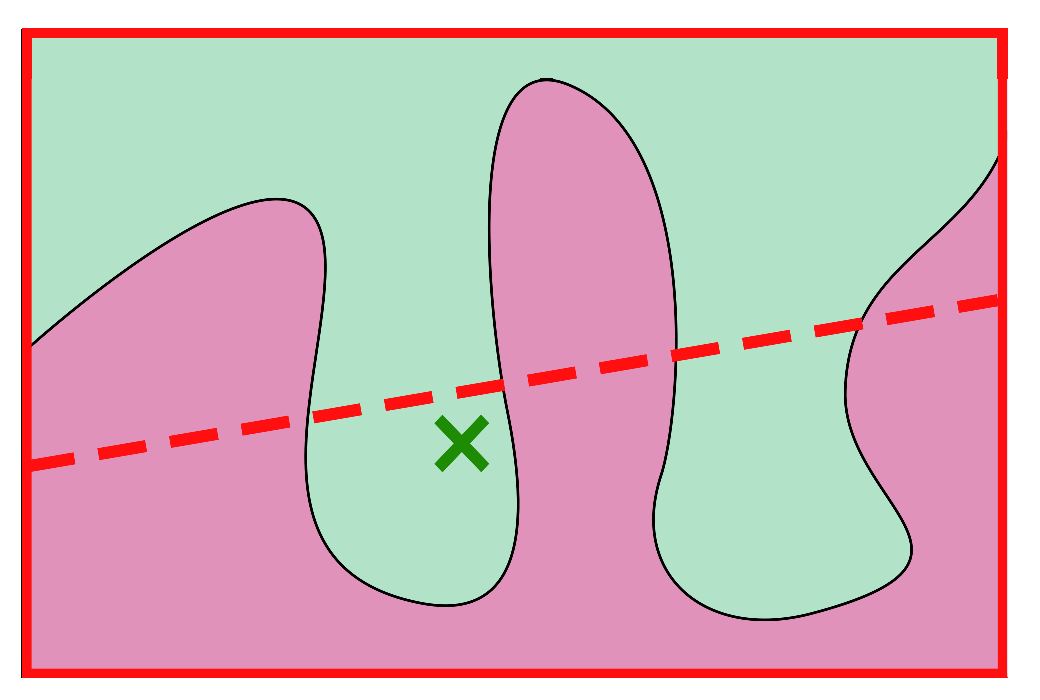
\includegraphics[width=0.32\textwidth]{visual-rlime1}
    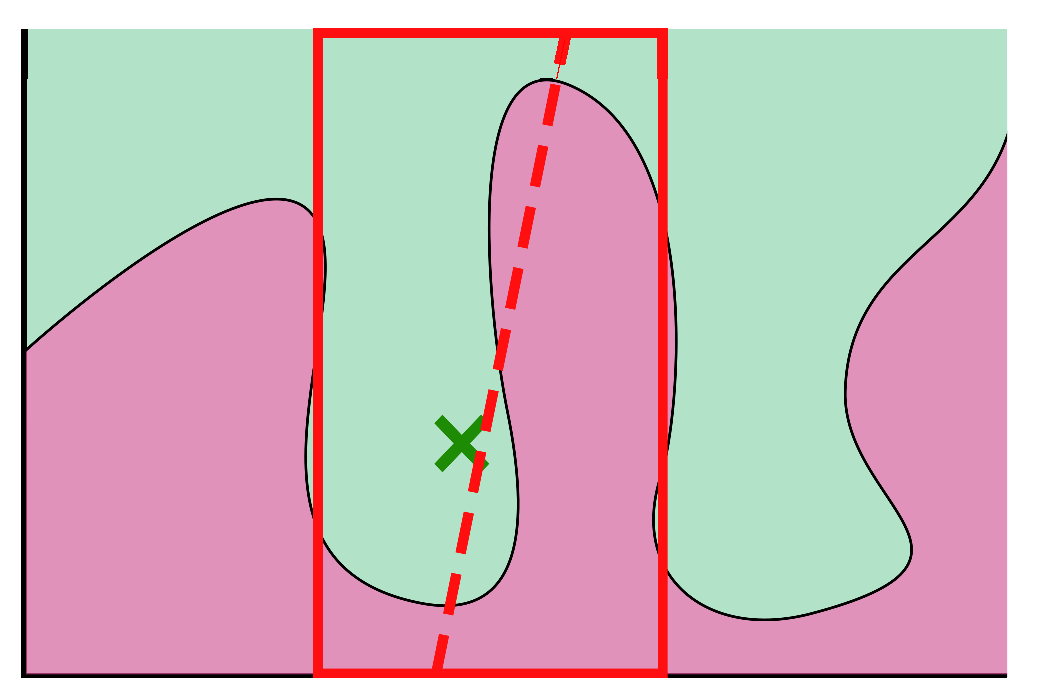
\includegraphics[width=0.32\textwidth]{visual-rlime2}
    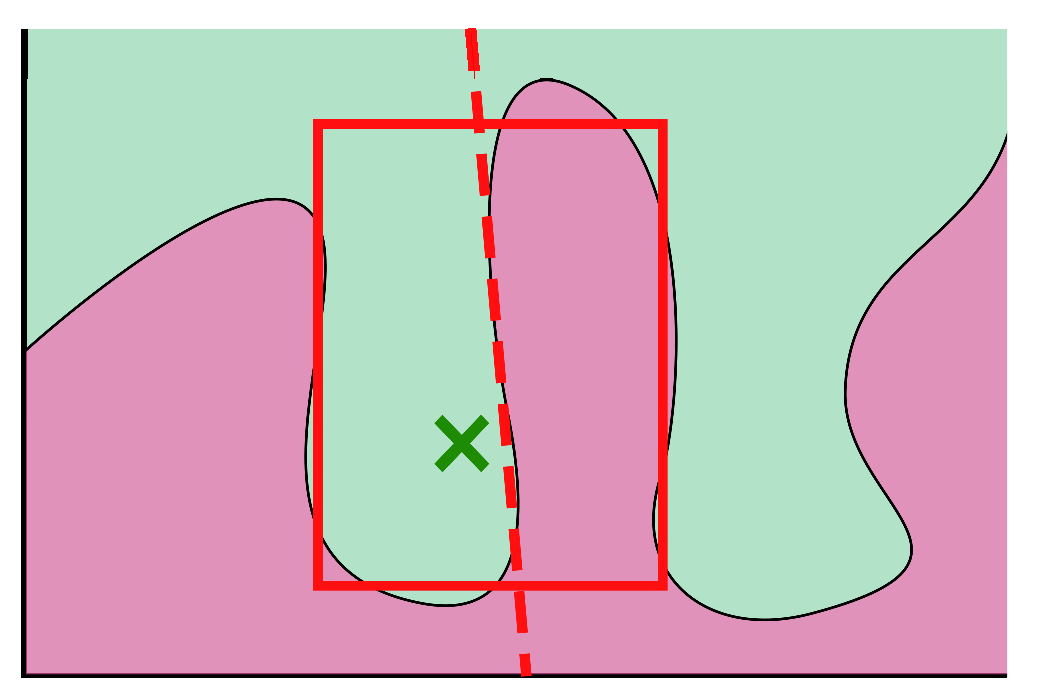
\includegraphics[width=0.32\textwidth]{visual-rlime3}
    \caption[Overview of the R-LIME algorithm]{%
      Overview of the R-LIME algorithm.
      The progression of the algorithm is illustrated from left to right.
      The solid line represents the rectangular region $A$,
      and the dashed line represents the linear approximation model $g$
      learned within $A$.
      The initial value of $A$ is an empty rule (entire input space),
      and predicates are added to $A$, reducing coverage.
      The process continues until $\Prec(A)\ge\tau$,
      at which point the rule with the maximum coverage is output.
    }
  \end{figure}
  \def\myidt{\hspace{\algorithmicindent}}
  \ifnum\mode=0
    \begin{algorithm}[t]
      \small
      \caption{R-LIME}\label{alg:greedy-search}
\begin{algorithmic}[1]
	\Require{%
		Black-box model $f$, Target instance $x$,
		Distribution $\mathcal{D}$,
		Threshold $\tau$, Beam width $B$, Tolerance $\epsilon$,
		Confidence level $1-\delta$
	}
	\Ensure{%
		Rule $A^*$ satisfying Eq.~\eqref{eq:main-problem}
	}
	\State{$A^*\gets\textbf{null},\ \mathcal{A}_0\gets\emptyset,\ t\gets0$}
	% \Comment{%
	%   Initialize the set of candidate rules $\mathcal{A}_0$ to $\emptyset$
	% }
	\Comment{Initialize the set of candidate rules $\mathcal{A}_0$ to $\emptyset$}
	\While{$A^*=\textbf{null}$}
	\State$t\gets t+1$
	\State$\cands_t\gets$ \Call{GenerateCands}
	{$\mathcal{A}_{t-1}$}
	\State$\mathcal{A}_t\gets$ \Call{B-BestCands}
	{$\cands_{t},\mathcal{D},B,\epsilon,\delta$}
	\State$A^*\gets$ \Call{LargestCand}
	{$\mathcal{A}_t,\tau,\delta$}
	\EndWhile%
\end{algorithmic}

    \end{algorithm}
  \else
    \begin{algorithm}[p]
      \small
      \caption{R-LIME}\label{alg:greedy-search}
\begin{algorithmic}[1]
	\Require{%
		Black-box model $f$, Target instance $x$,
		Distribution $\mathcal{D}$,
		Threshold $\tau$, Beam width $B$, Tolerance $\epsilon$,
		Confidence level $1-\delta$
	}
	\Ensure{%
		Rule $A^*$ satisfying Eq.~\eqref{eq:main-problem}
	}
	\State{$A^*\gets\textbf{null},\ \mathcal{A}_0\gets\emptyset,\ t\gets0$}
	% \Comment{%
	%   Initialize the set of candidate rules $\mathcal{A}_0$ to $\emptyset$
	% }
	\Comment{Initialize the set of candidate rules $\mathcal{A}_0$ to $\emptyset$}
	\While{$A^*=\textbf{null}$}
	\State$t\gets t+1$
	\State$\cands_t\gets$ \Call{GenerateCands}
	{$\mathcal{A}_{t-1}$}
	\State$\mathcal{A}_t\gets$ \Call{B-BestCands}
	{$\cands_{t},\mathcal{D},B,\epsilon,\delta$}
	\State$A^*\gets$ \Call{LargestCand}
	{$\mathcal{A}_t,\tau,\delta$}
	\EndWhile%
\end{algorithmic}

    \end{algorithm}
  \fi

  \foreach \alg in {2,3,4}{%
      \begin{algorithm}[p]
        \small
        \input{tex/alg\alg}
      \end{algorithm}
    }
}
The algorithm of R-LIME
is mainly based on that used in Anchor\cite{ribeiro2018anchors}.
For non-convex optimization problems like \cref{eq:main_problem},
greedy search are often used.
However,
greedy methods tend to converge to local optima, and to address this,
R-LIME utilizes beam search,
which selects multiple candidates at each iteration.
The pseudo code is shown in \cref{alg:greedy_search}.

\subsubsection{Generation of New Candidate Rules}
To generate new candidate rules,
one additional predicate is added to each of the $B$ candidate rules
selected in the previous iteration.
The pseudo code is shown in \cref{alg:generate_cands}.
$T(x)$ is the set of attribute-value pairs (predicates) that are true for $x$,
and $T(x)\setminus A$ is the set of predicates in $T(x)$ not included in rule $A$.

\subsubsection{Selection of Candidate Rules with Maximum Accuracy}
Given the set of candidate rules $\cands$,
the algorithm selects the top $B$ candidates with the highest accuracy.
This problem can be formulated
as best arm identification in the multi-armed bandit framework.
Each candidate rule $A_i\in\cands$ is considered as an arm,
and its accuracy $\Prec(A_i)$ is considered as the distribution of rewards.
By sampling $z\sim\mathcal{D}(\cdot|A_i)$
and obtaining the reward $\mathbbm{1}_{f(z)=g_i(z)}$ for each trial,
the algorithm updates $g_i$ using the sampled perturbation vector $z$
and the pseudo-label $f(z)$ after each trial.
To efficiently select the rule (arm) with the highest accuracy,
we employ the KL-LUCB algorithm \cite{kaufmann2013information}.
The pseudo code is shown in \cref{alg:best_cands}.
For tolerance $\epsilon\in[0,1]$, the KL-LUCB algorithm guarantees below:
\begin{equation}
  P(\underset{A\in\cands}{\min}\Prec(A)\ge
  \underset{A'\in\mathcal{A}}{\min}\Prec(A')-\epsilon)\ge1-\delta.
\end{equation}
However,
the KL-LUCB algorithm assumes that the reward distribution for each arm
remains unchanged,
while our method updates the classifier $g_i$ with each sampling,
which may not satisfy this assumption.
This issue is discussed further in \cref{sec:reward}.

\subsubsection{Selection of the Rule with Maximum Coverage Meeting the Constraint}
To satisfy the constraint imposed by \cref{eq:const_prec}, rule $A$ needs to fulfill the lower bound constraint:
\begin{equation}
  \Prec_{l}(A,\delta)>\tau
  \label{eq:stop_condition}
\end{equation}
where $\Prec_{l}(A,\delta)$ is the lower limit of
the $100(1-\delta)$\% confidence interval for $\Prec(A)$.
If the received set of candidate rules, $\mathcal{A}$,
includes a rule satisfying \cref{eq:stop_condition},
the one with the maximum coverage among them is selected,
and the iteration is terminated.
If $\mathcal{A}$ does not contain any rule satisfying \cref{eq:stop_condition},
it returns \textbf{null},
and proceeds to the next iteration.
The pseudo code is presented in \cref{alg:largest_valid_cand}.

% The algorithmic procedure outlined above approximates
% the solution to the optimization problem in \cref{eq:main_problem}
% under the definition of accuracy in \cref{eq:def_prec}. 

\ifnum\mode=1
  \subsection{Computational Complexity}
  Post-hoc explanation methods including LIME, Anchor, and R-LIME
  need to sample a perturbation vector
  and get the output of the black-box model multiple times,
  which is computationally expensive.
  The number of samples required for LIME is $|\mathcal{Z}_p|$,
  which is the number of samples designated by the user.
  On the other hand,
  the expected number of samples required for Anchor and R-LIME is bounded by
  $\mathcal{O}[m\cdot\mathcal{O}_{\mathrm{MAB}[B\cdot m,B]}]$,
  where $\mathcal{O}_{\mathrm{MAB}[B\cdot m,B]}$
  is the expected number of samples
  for best arm identification finding the best $B$ arms from $B\cdot m$ arms.
  For KL-LUCB algorithm~\cite{kaufmann2013information},
  \begin{equation}
    \mathcal{O}_{\mathrm{MAB}[B\cdot m,B]}=
    \mathcal{O}\left[\frac{Bm}{\epsilon^2}\log\frac{Bm}{\epsilon^2\delta}\right].
  \end{equation}
  Then the total expected number of samples for Anchor and R-LIME is bounded by
  \begin{equation}
    \mathcal{O}\left[\frac{Bm^2}{\epsilon^2}\log\frac{Bm}{\epsilon^2\delta}\right].
  \end{equation}

  For each iteration of KL-LUCB algorithm, R-LIME needs to update
  the linear classifier $g_i$, which is not required in Anchor.
  But if we use logistic regression as the linear classifier,
  the computational complexity of updating $g_i$ is $\mathcal{O}(m)$,
  which is negligible compared to the complexity of sampling a perturbation vector
  and getting the output of the black-box model.
  Overall, the computational complexity of R-LIME is comparable to that of Anchor.
\fi

\section{Experiments}
To verify the effectiveness of the proposed method,
We compare LIME and R-LIME using a real-world dataset.

\subsection{Qualitative Evaluation}
\subsubsection{Experimental Setup}\label{sec:exp_setting}
{%
  \renewcommand{\arraystretch}{1.05}
  \begin{table}[tbp]
    \centering
    \caption[Attributes of the recidivism dataset used in the experiments]{%
      Attributes of the recidivism dataset used in the experiments.
      Continuous features are all discretized,
      and only binary and ordinal features are considered.
    }\label{tab:rcdv}
    \ifnum\mode=0
      \small
    \fi
    \begin{tabular}{llc}
      \toprule
      Attribute              & Overview                              & \# of \ifnum\mode=1 Possible \fi Values \\
      \midrule
      Race                   & Race (Black or White)                 & 2                                       \\
      Alcohol                & Presence of serious alcohol issues    & 2                                       \\
      Junky                  & Drug usage                            & 2                                       \\
      Supervised Release     & Supervised release                    & 2                                       \\
      Married                & Marital status                        & 2                                       \\
      Felony                 & Felony or not                         & 2                                       \\
      WorkRelease            & Participation in work release program & 2                                       \\
      Crime against Property & Crime against property or not         & 2                                       \\
      Crime against Person   & Crime against a person or not         & 2                                       \\
      Gender                 & Gender (Female or Male)               & 2                                       \\
      Priors                 & Number of prior offenses              & 4                                       \\
      YearsSchool            & Years of formal education completed   & 4                                       \\
      PrisonViolations       & Number of prison rule violations      & 3                                       \\
      Age                    & Age                                   & 4                                       \\
      MonthsServed           & Months served in prison               & 4                                       \\
      \midrule
      Recidivism             & Recidivism or not                     & 2                                       \\
      \bottomrule
    \end{tabular}
  \end{table}
}

The experiments utilized the recidivism dataset \cite{schmidt1988predicting}.
This dataset contains information on 9,549 prisoners released from
North Carolina prisons between July 1, 1979, and June 30, 1980.
The dataset includes 19 items such as race, gender,
presence of alcohol dependence, number of prior offenses and recidivism.
For this experiment,
we treated the binary classification problem of predicting
the presence or absence of recidivism (Recidivism) as the target label.
We discretized continuous features and removed missing values,
resulting in 15 features.
This problem setting can be considered as a case
where a machine learning model is introduced to decide parole for prisoners.
Since such decisions can have a significant impact on a person's life,
it is crucial for users to interpret the outputs of black-box models appropriately.

The dataset, after removing missing values,
was split into training data (7,639 instances) and test data (955 instances).
A random forest model with 50 trees was trained using the training data.
Subsequently, LIME and R-LIME explanations were generated
for two instances extracted from the test data (\cref{fig:instance}).
For R-LIME, logistic regression was used as the linear approximation model,
and the distribution $\mathcal{D}$ was a multivariate normal distribution
estimated from the training data.
The beam width was set to $B=10$,
the confidence coefficient to $1-\delta=0.95$,
and the tolerance of the KL-LUCB algorithm to $\epsilon=0.05$.
Accuracy thresholds $\tau$ were set to $\tau=0.70,0.80,0.90$.

  {%

    \def\dir{experiments/exp1}
    \def\Asample{0012}
    \def\Bsample{0011}
    \def\index#1{\ifnum#1=0 \Asample \else \Bsample \fi}

    {%
      \def\AB#1{\ifnum#1=0 A\else B\fi}
      \def\mylabel#1{\ifnum#1=0 \label{fig:A-instance}\else \label{fig:B-instance}\fi}
      \ifnum\mode=0
        \renewcommand{\arraystretch}{0.97}
      \else
        \renewcommand{\arraystretch}{1.02}
      \fi
      \begin{figure}[tbp]
        \foreach\a in {0,1}{%
            \centering
            \begin{subfigure}{\textwidth}
              \ifnum\mode=0
                \small
              \fi
              \centering
              \begin{tabular}{p{14em}m{16em}}
                \toprule
                \csvreader[no head, late after line= \\]{%
                  \dir/\index{\a}.csv
                }{}{%
                \ifnum\thecsvrow=16 \midrule\fi\csvcoli & \csvcolii
                }
                \bottomrule
              \end{tabular}
              \caption{Instance~\AB{\a}}\mylabel{\a}
              \vspace{15pt}
            \end{subfigure}
          }
        \vspace{-15pt}
        \caption[Two instances sampled from recidivism dataset]{%
          Two instances sampled from recidivism dataset.
        }\label{fig:instance}
      \end{figure}
    }
    {%
      \ifnum\mode=0
        \def\scale{0.32}
        \def\imgwidth{0.45\textwidth}
        \def\hspacebase{\hspace{-0.5em}}
      \else
        \def\scale{0.315}
        \def\imgwidth{0.495\textwidth}
        \def\hspacebase{\hspace{-1.5em}}
      \fi
      \def\vspacebase{\vspace{0.5em}}
      \def\vspacebeforecaption{\vspace{-0.4em}}
      \begin{figure}[p]
        \centering
        \begin{subfigure}[t]{\imgwidth}
          \hspacebase
          \hspace{1.0em}
          \includegraphics[scale=\scale]{\dir/lime-\Asample}
          \vspacebeforecaption
          \caption{LIME}\label{fig:A-lime}
          \vspacebase
        \end{subfigure}
        \begin{subfigure}[t]{\imgwidth}
          \hspacebase
          \hspace{0.5em}
          \includegraphics[scale=\scale]{\dir/newlime-\Asample-70}
          \vspacebeforecaption
          \caption{R-LIME ($\tau=0.70$)}\label{fig:A-rlime-70}
          \vspacebase
        \end{subfigure}
        \begin{subfigure}[t]{\imgwidth}
          \hspacebase
          \includegraphics[scale=\scale]{\dir/newlime-\Asample-80}
          \vspacebeforecaption
          \caption{R-LIME ($\tau=0.80$)}\label{fig:A-rlime-80}
        \end{subfigure}
        \begin{subfigure}[t]{\imgwidth}
          \hspacebase
          \hspace{-0.5em}
          \includegraphics[scale=\scale]{\dir/newlime-\Asample-90}
          \vspacebeforecaption
          \caption{R-LIME ($\tau=0.90$)}\label{fig:A-rlime-90}
        \end{subfigure}
        \caption[Explanation for Instance A by LIME and R-LIME]{%
          Explanation for Instance A by LIME and R-LIME.
        }\label{fig:A}
      \end{figure}
      \begin{figure}[p]
        \centering
        \begin{subfigure}[t]{\imgwidth}
          \hspacebase
          \hspace{-0.7em}
          \includegraphics[scale=\scale]{\dir/lime-\Bsample}
          \vspacebeforecaption
          \caption{LIME}\label{fig:B-lime}
          \vspacebase
        \end{subfigure}
        \begin{subfigure}[t]{\imgwidth}
          \hspacebase
          \hspace{0.5em}
          \includegraphics[scale=\scale]{\dir/newlime-\Bsample-70}
          \vspacebeforecaption
          \caption{R-LIME ($\tau=0.70$)}\label{fig:B-rlime-70}
          \vspacebase
        \end{subfigure}
        \begin{subfigure}[t]{\imgwidth}
          \hspacebase
          \hspace{-0.8em}
          \includegraphics[scale=\scale]{\dir/newlime-\Bsample-80}
          \vspacebeforecaption
          \caption{R-LIME ($\tau=0.80$)}\label{fig:B-rlime-80}
        \end{subfigure}
        \begin{subfigure}[t]{\imgwidth}
          \hspacebase
          \hspace{-0.8em}
          \includegraphics[scale=\scale]{\dir/newlime-\Bsample-90}
          \vspacebeforecaption
          \caption{R-LIME ($\tau=0.90$)}\label{fig:B-rlime-90}
        \end{subfigure}
        \caption[Explanation for Instance B by LIME and R-LIME]{%
          Explanation for Instance B by LIME and R-LIME.
        }\label{fig:B}
      \end{figure}
    }
  }
\subsubsection{Experimental Results}
The results of the experiment are shown in \cref{fig:A,fig:B}.
The values assigned to each attribute name represent the contribution
(weights of the learned linear classifier)
to the output of the black-box classifier,
normalized such that the absolute sum is 1.
The figures also display the 5 attributes with the highest absolute contribution.

Explanations generated by LIME (\cref{fig:A-lime,fig:B-lime}) provide insights
that attributes such as having a prior offenses (Priors),
being served for a long time in prison (MonthsServed),
and committing a crime against property (Crime against Property)
primarily contribute to the positive prediction
(prediction that the prisoner will be re-arrested).
On the other hand,
attributes like older age (Age), being married (Married),
and being of white race (Race) contribute to the negative prediction
(prediction that the prisoner will not be re-arrested).
While these LIME explanations provide valuable insights into the behavior of
the black-box model,
they do not explicitly indicate the application scope of the explanations,
leaving users unable to determine to which inmates the explanations are applicable.

In contrast, R-LIME expresses the application scope of explanations
as a conjunction of predicates.
For example, the explanation for instance A
under $\tau=0.70$ (\cref{fig:A-rlime-70}) indicates that it is applicable
only to married prisoner (Married$=$Yes).
Furthermore, the explanations include the accuracy and coverage,
allowing users to evaluate its reliability.
For example, the coverage of the explanation for instance B under $\tau=0.90$
(\cref{fig:B-rlime-90}) is 0.01\%,
indicating that the decision boundaries around instance B are complex,
making it challenging to obtain a high-accuracy linear approximation.
This allows users to discern that the application scope of this explanation is
very narrow, limiting its utility.

\subsection{Quantitative Evaluation}\label{sec:exp2}
\subsubsection{Experimental Setup}
To demonstrate that R-LIME learns a highly accurate linear approximation model
in the optimized approximation region,
we conducted a comparison of the local accuracy of explanations
between LIME and R-LIME\@.
Using the same settings as in \cref{sec:exp_setting},
we randomly sampled 100 instances from the test data of the recidivism dataset
and generated explanations (with $\tau=0.70,0.80,0.90$) using LIME and R-LIME\@.
We then sampled 10,000 instances within the rectangular region
obtained by R-LIME and calculated the local accuracy of both methods.
\subsubsection{Experimental Results}
\begin{figure}[tbp]
  \centering
  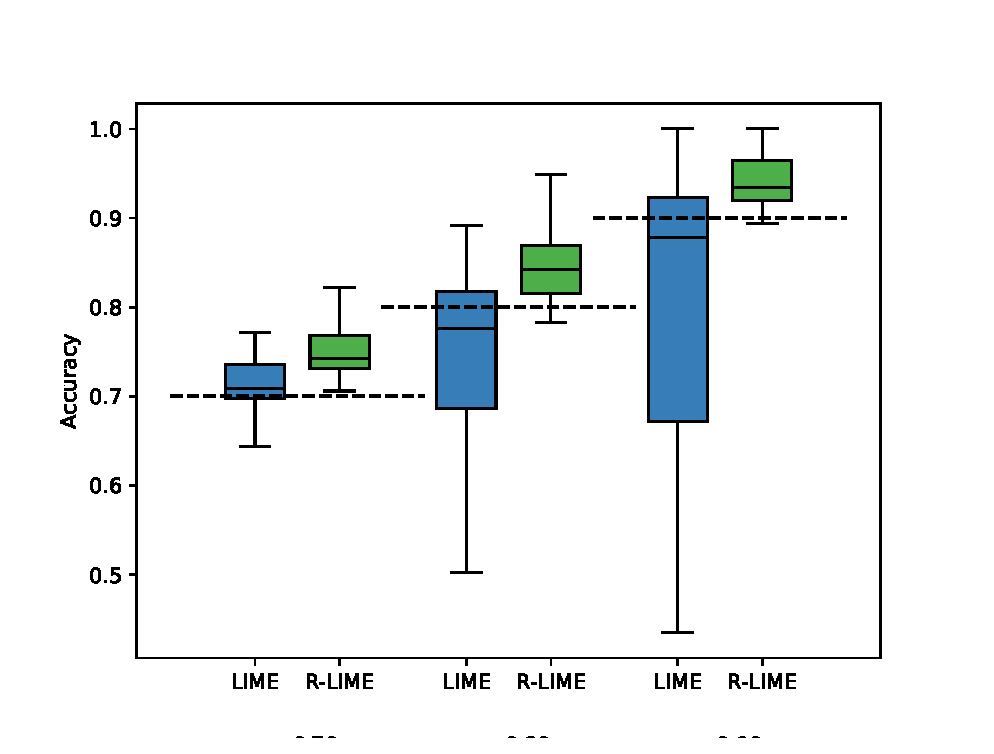
\includegraphics[width=0.5\textwidth]{experiments/exp2/box_plot}
  \caption[Comparison of Local Accuracy between R-LIME and LIME]{%
    Comparison of local accuracy between LIME and R-LIME\@.
    R-LIME achieved higher and less variable accuracy compared to LIME
    for all values of $\tau$.
  }\label{fig:box_plot}
\end{figure}
The results are presented in \cref{fig:box_plot},
showing the distribution of the accuracy of the linear approximation models
learned by LIME and R-LIME\@.
R-LIME achieved higher accuracy compared to LIME for all values of $\tau$.
This suggests that the linear classifiers learned by LIME and R-LIME
differ significantly,
and R-LIME learns a high-accuracy linear classifier adapted to the rectangular region.
Additionally, as $\tau$ increases,
the variability in the accuracy of LIME widens.
This indicates that the linear classifiers learned by LIME may not function
effectively as approximation models depending on how the region is selected.

\section{Challenges and Future Work}
 {%
  \def\imgwidth{0.47\textwidth}
  \begin{figure}[t]
    \centering
    \begin{subfigure}[t]{\imgwidth}
      \centering
      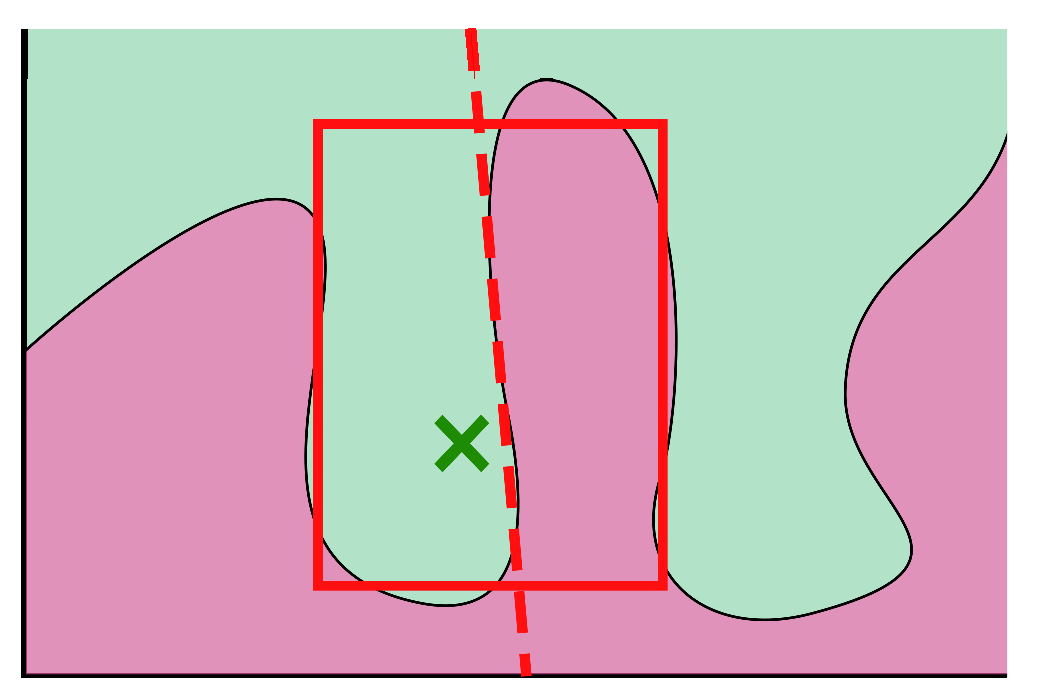
\includegraphics[width=0.7\textwidth]{visual-rlime3}
      \caption{R-LIME for balanced label distribution.}\label{fig:balanced}
    \end{subfigure}
    \begin{subfigure}[t]{\imgwidth}
      \centering
      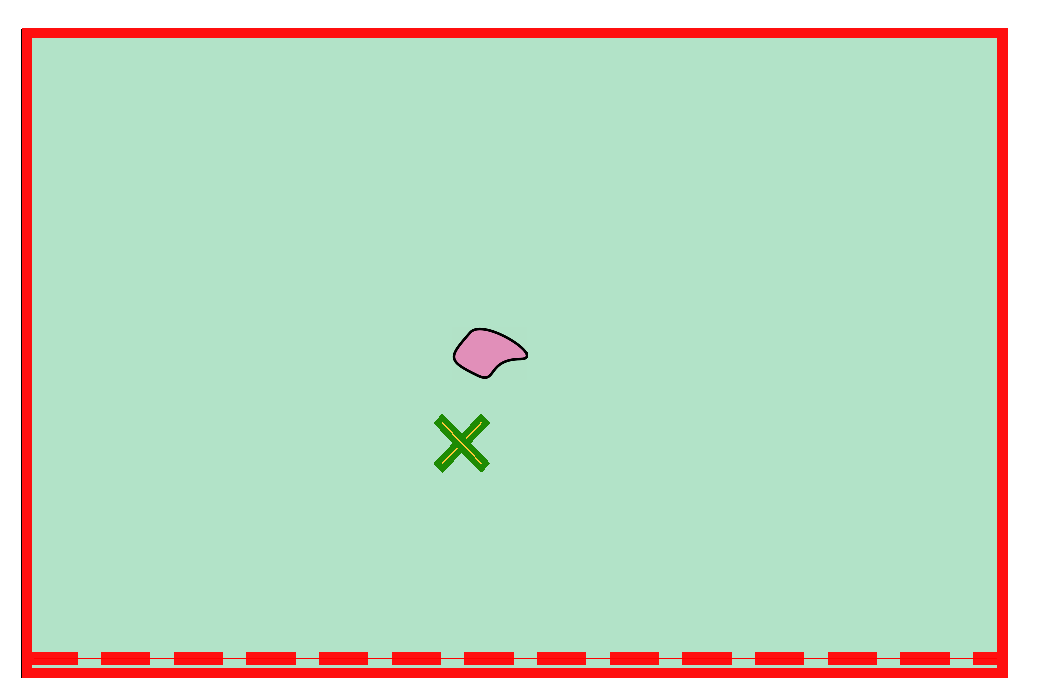
\includegraphics[width=0.7\textwidth]{visual-rlime-imbalanced}
      \caption{R-LIME for imbalanced label distribution.
      }\label{fig:imbalanced}
    \end{subfigure}
    \caption[Behavior of R-LIME for balanced and imbalanced label distribution]{%
      Behavior of R-LIME for balanced and imbalanced label distribution.
      In case of imbalanced label distribution,
      the approximation region covers the entire input space and the
      linear approximation model always outputs the majority label.
    }
  \end{figure}
 }

\subsection{Behavior Regarding Imbalanced Label Distribution}
R-LIME may generate less useful explanations
when there is bias in the distribution of black-box model outputs.
When the distribution of black-box model outputs is significantly biased
for a given accuracy threshold $\tau$
(when the ratio of the minority label is less than $1-\tau$),
the approximation region generated by R-LIME covers the entire input space,
and the learned linear classifier always outputs the majority label
(\cref{fig:imbalanced}).

A first possible solution to this problem is modifying the loss function.
Using weighted logistic loss or Focal Loss \cite{lin2020focal}
as the loss function might lead to the generation of more useful explanations
in the case of imbalanced label distribution.
Another solution involves adding constraints
to limit the label distribution bias within the approximation region.
In addition to \cref{eq:const_prec}, adding a constraint like
\begin{equation}
  {%
    \left(
    \mathbb{E}_{z\sim\mathcal{D}(z\mid A)}[\mathbbm{1}_{f(z)=1}]-\frac{1}{2}
    \right)
  }^2<\mu
\end{equation}
could suppress the excessive expansion of the approximation region.

\subsection{Changes in Reward Distribution in Best Arm Identification}\label{sec:reward}
{%
  \renewcommand{\arraystretch}{1.1}
  \begin{table}[tbp]
    \centering
    \caption[Deviation between the estimated accuracy and the true accuracy]{%
      Deviation between the estimated accuracy and the true accuracy.
      Deviation was relatively small considering confidence level $1-\delta=0.95$.
    }\label{tab:reward}
    \begin{tabular}{cccc}
  \toprule
                     & Estimated acc. & True acc. & Deviation \\
  \midrule
  Average            & .811           & .829      & .012      \\
  Standard Deviation & .018           & .023      & .017      \\
  \bottomrule
\end{tabular}

  \end{table}
}
For R-LIME,
the problem of selecting the rule with the highest accuracy is formulated
as the optimal arm identification problem in multi-armed bandit theory,
solved using the KL-LUCB algorithm \cite{kaufmann2013information}.
However, this algorithm assumes that the reward distribution remains constant,
while in R-LIME,
the reward distribution (accuracy of the linear approximation)
changes with every update of the approximation model after sampling.
Therefore, rewards obtained at an early stage
might influence the estimated value and deviate from the true value.

We conducted an experiment to evaluate the deviation
between the estimated accuracy and the true accuracy.
We generated explanations for 3,200 data instances sampled from the dataset,
and compared the estimated accuracy with the true accuracy.
The true accuracy was calculated based on 1,000 instances sampled
within the approximation region.
The results in \cref{tab:reward} show a mean deviation of 0.012
with a standard deviation of 0.017.
By considering the confidence level $1-\delta=0.95$,
the deviation was relatively small.
While there are concerns about the theoretical validity of using the KL-LUCB algorithm,
the results suggest that the deviation is not significant in practice.

\section{Conclusion}
Existing methods for
local model-agnostic explanations of black-box classifiers have limitations
that they do not explicitly indicate the application scope of the explanations.
To address these challenges,
we proposed R-LIME, a method that locally approximates the decision boundary
of a black-box classifier linearly and provides a rectangular approximation region,
which is interpretable for users due to being expressed as a conjunction of feature predicates.
We proposed an algorithm to
maximize coverage of the approximation region
as long as the accuracy of the linear approximation model exceeds a given threshold.
Comparing the outputs of LIME and R-LIME on the real-world dataset,
we demonstrated that R-LIME provides a clear application scope of the
explanation, can be evaluated by users for its reliability and generality,
and achieves higher and less variable local accuracy compared to LIME\@.
However, we discussed the instability of behavior against imbalanced label
distributions and raised questions about the theoretical validity of using
the KL-LUCB algorithm for our problem.

\ifnum\mode=0
  \acknowledge
  I would like to thank Associate Professor Keigo Kimura
  of the Laboratory for Pattern Recognition and Machine Learning,
  Division of Computer Science and Information Technology,
  Graduate School of Information Sci.\ and Tech., Hokkaido University.
  He provided valuable guidance
  from setting the research theme to outlining the research method.
  Furthermore,
  I appreciate the various insights shared by Professor Mineichi Kudo
  in the same laboratory.
  Finally, I am deeply thankful to all the members of our laboratory
  for their helpful advice and cooperation throughout the research process.
\fi

\ifnum\mode=0
  \bibliographystyle{style/prml}
\else
  \bibliographystyle{style/splncs04}
\fi
\bibliography{myref/myref}

\end{document}
